\documentclass{ltjsarticle}
\usepackage{tikz}
\usetikzlibrary{positioning,calc,intersections}

\begin{document}
\begin{center}
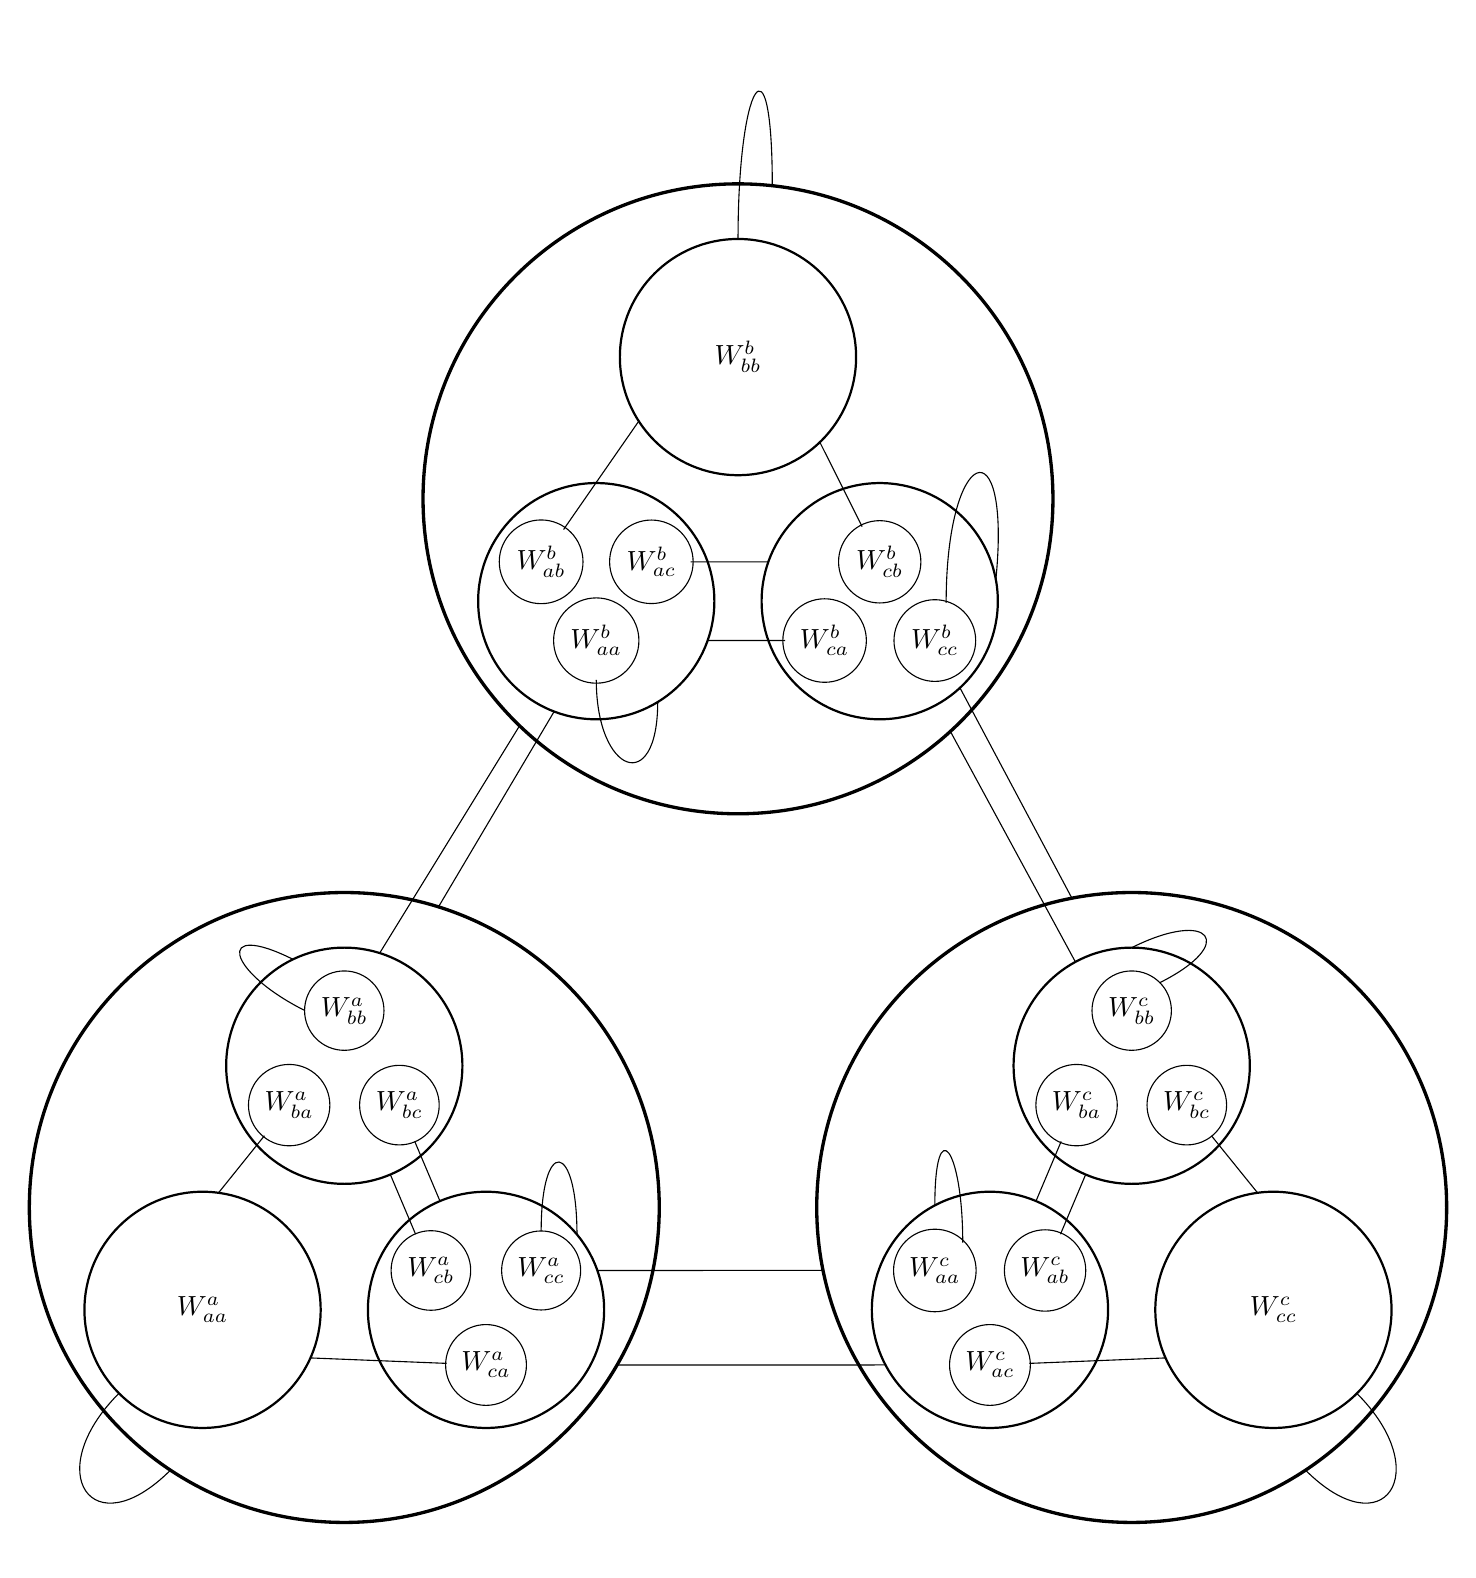
\begin{tikzpicture}[
    outer circle/.style={circle, draw, line width=1.2pt, minimum size=8cm},
    middle circle/.style={circle, draw, line width=0.8pt, minimum size=3cm},
    inner circle/.style={circle, draw, line width=0.4pt, minimum size=1cm}
]
    % 大円A
    \node[outer circle] (A) at (-7,-5) {};
    % Aの中円と小円
    \node[middle circle] (A1) at ($(A) + (0,1.8)$) {};
    \node[inner circle] (A13) at ($(A1) + (0,0.7)$) {$W_{bb}^{a}$};
    \node[inner circle] (A12) at ($(A1) + (-0.7,-0.5)$) {$W_{ba}^{a}$};
    \node[inner circle] (A11) at ($(A1) + (0.7,-0.5)$) {$W_{bc}^{a}$};

    \node[middle circle] (A2) at ($(A) + (-1.8,-1.3)$) {$W_{aa}^{a}$};

    \node[middle circle] (A3) at ($(A) + (1.8,-1.3)$) {};
    \node[inner circle] (A31) at ($(A3) + (0,-0.7)$) {$W_{ca}^{a}$};
    \node[inner circle] (A32) at ($(A3) + (-0.7,0.5)$) {$W_{cb}^{a}$};
    \node[inner circle] (A33) at ($(A3) + (0.7,0.5)$) {$W_{cc}^{a}$};

    % 大円B
    \node[outer circle] (B) at (-2,4) {};
    % Bの中円と小円
    \node[middle circle] (B1) at ($(B) + (0,1.8)$) {$W_{bb}^{b}$};

    \node[middle circle] (B2) at ($(B) + (-1.8,-1.3)$) {};
    \node[inner circle] (B22) at ($(B2) + (0,-0.5)$) {$W_{aa}^{b}$};
    \node[inner circle] (B23) at ($(B2) + (-0.7,0.5)$) {$W_{ab}^{b}$};
    \node[inner circle] (B21) at ($(B2) + (0.7,0.5)$) {$W_{ac}^{b}$};

    \node[middle circle] (B3) at ($(B) + (1.8,-1.3)$) {};
    \node[inner circle] (B31) at ($(B3) + (0,0.5)$) {$W_{cb}^{b}$};
    \node[inner circle] (B32) at ($(B3) + (-0.7,-0.5)$) {$W_{ca}^{b}$};
    \node[inner circle] (B33) at ($(B3) + (0.7,-0.5)$) {$W_{cc}^{b}$};

    % 大円C
    \node[outer circle] (C) at (3,-5) {};
    % Cの中円と小円
    \node[middle circle] (C1) at ($(C) + (0,1.8)$) {};
    \node[inner circle] (C13) at ($(C1) + (0,0.7)$) {$W_{bb}^{c}$};
    \node[inner circle] (C11) at ($(C1) + (-0.7,-0.5)$) {$W_{ba}^{c}$};
    \node[inner circle] (C12) at ($(C1) + (0.7,-0.5)$) {$W_{bc}^{c}$};

    \node[middle circle] (C2) at ($(C) + (-1.8,-1.3)$) {};
    \node[inner circle] (C22) at ($(C2) + (0,-0.7)$) {$W_{ac}^{c}$};
    \node[inner circle] (C23) at ($(C2) + (-0.7,0.5)$) {$W_{aa}^{c}$};
    \node[inner circle] (C21) at ($(C2) + (0.7,0.5)$) {$W_{ab}^{c}$};

    \node[middle circle] (C3) at ($(C) + (1.8,-1.3)$) {$W_{cc}^{c}$};


\path[name path = cA]  (A) circle (4cm);
\path[name path = cB]  (B) circle (4cm);
\path[name path = cC]  (C) circle (4cm);
\path[name path = cA1]  (A1) circle (1.5cm);          % A1を中心とする円
\path[name path = cA2]  (A2) circle (1.5cm);
\path[name path = cA3]  (A3) circle (1.5cm);
\path[name path = cB1]  (B1) circle (1.5cm);
\path[name path = cB2]  (B2) circle (1.5cm);
\path[name path = cB3]  (B3) circle (1.5cm);
\path[name path = cC1]  (C1) circle (1.5cm);
\path[name path = cC2]  (C2) circle (1.5cm);
\path[name path = cC3]  (C3) circle (1.5cm);
\path[name path = cA11]  (A11) circle (0.5cm);          % A13を中心とする円
\path[name path = cA12]  (A12) circle (0.5cm);
\path[name path = cA13]  (A13) circle (0.5cm);
\path[name path = cA31]  (A31) circle (0.5cm);
\path[name path = cA32]  (A32) circle (0.5cm);
\path[name path = cA33]  (A33) circle (0.5cm);
\path[name path = cB21]  (B21) circle (0.5cm);          % A13を中心とする円
\path[name path = cB22]  (B22) circle (0.5cm);
\path[name path = cB23]  (B23) circle (0.5cm);
\path[name path = cB31]  (B31) circle (0.5cm);
\path[name path = cB32]  (B32) circle (0.5cm);
\path[name path = cB33]  (B33) circle (0.5cm);
\path[name path = cC11]  (C11) circle (0.5cm);          % A13を中心とする円
\path[name path = cC12]  (C12) circle (0.5cm);
\path[name path = cC13]  (C13) circle (0.5cm);
\path[name path = cC21]  (C21) circle (0.5cm);
\path[name path = cC22]  (C22) circle (0.5cm);
\path[name path = cC23]  (C23) circle (0.5cm);


\path[name path = line1] (A13.center) -- (B2.center);  % 円の中心間のパス
\path[name intersections = {of = line1 and cA1, by = P1}];  % 交点をP1と名付ける
\path[name intersections = {of = line1 and cB, by = Q9}];
\path[name path = line2] (A1.center) -- (B22.center);  % 円の中心間のパス
\path[name intersections = {of = line2 and cB2, by = Q8}]; 
\path[name intersections = {of = line2 and cA, by = P11}]; 

\path[name path = line3] (A33.center) -- (C23.center);
\path[name intersections = {of = line3 and cA3, by = P10}]; 
\path[name intersections = {of = line3 and cC, by = R12}];
\path[name path = line4] (A31.center) -- (C22.center);
\path[name intersections = {of = line4 and cC2, by = R11}]; 
\path[name intersections = {of = line4 and cA, by = P12}];

\path[name path = line5] (C13.center) -- (B33.center);
\path[name intersections = {of = line5 and cB3, by = Q10}]; 
\path[name intersections = {of = line5 and cC, by = R1}];
\path[name path = line6] (C1.center) -- (B3.center);
\path[name intersections = {of = line6 and cB, by = Q11}]; 
\path[name intersections = {of = line6 and cC1, by = R2}];

\path[name path = line7] (B22.center) -- (B32.center);
\path[name intersections = {of = line7 and cB2, by = Q7}]; 
\path[name intersections = {of = line7 and cB32, by = Q6}];
\path[name path = line8] (B21.center) -- (B31.center);
\path[name intersections = {of = line8 and cB21, by = Q4}]; 
\path[name intersections = {of = line8 and cB3, by = Q5}];

\path[name path = line9] (A32.center) -- (A1.center);
\path[name intersections = {of = line9 and cA1, by = P5}]; 
\path[name intersections = {of = line9 and cA32, by = P6}];
\path[name path = line10] (A11.center) -- (A3.center);
\path[name intersections = {of = line10 and cA11, by = P4}]; 
\path[name intersections = {of = line10 and cA3, by = P7}];

\path[name path = line11] (C11.center) -- (C2.center);
\path[name intersections = {of = line11 and cC11, by = R3}]; 
\path[name intersections = {of = line11 and cC2, by = R4}];
\path[name path = line12] (C21.center) -- (C1.center);
\path[name intersections = {of = line12 and cC21, by = R5}]; 
\path[name intersections = {of = line12 and cC1, by = R6}];

\path[name path = line13] ($(A2.center) + (-1.4cm,-0.5cm)$) -- (A31.center);
\path[name intersections = {of = line13 and cA31, by = P9}]; 
\path[name intersections = {of = line13 and cA2, by = P8}];
\path[name path = line14] ($(A2.center) + (-1.4cm,-0.5cm)$) -- (A12.center);
\path[name intersections = {of = line14 and cA12, by = P2}]; 
\path[name intersections = {of = line14 and cA2, by = P3}];

\path[name path = line15] ($(C3.center) + (+1.4cm,-0.5cm)$) -- (C12.center);
\path[name intersections = {of = line15 and cC12, by = R7}]; 
\path[name intersections = {of = line15 and cC3, by = R8}];
\path[name path = line16] ($(C3.center) + (+1.4cm,-0.5cm)$) -- (C22.center);
\path[name intersections = {of = line16 and cC22, by = R9}]; 
\path[name intersections = {of = line16 and cC3, by = R10}];

\path[name path = line17]  ($(B1.center) + (0,1cm)$)  -- (B23.center);
\path[name intersections = {of = line17 and cB1, by = Q1}]; 
\path[name intersections = {of = line17 and cB23, by = Q3}];
\path[name path = line18]  ($(B1.center) + (0,1cm)$)  -- (B31.center);
\path[name intersections = {of = line18 and cB1, by = Q2}]; 
\path[name intersections = {of = line18 and cB31, by = Q12}];

\path[name path = line19]  (A13.center)  -- ($(A13.center)+(-1cm,0)$);
\path[name intersections = {of = line19 and cA13, by = P13}]; 
\path[name path = line20]  (A13.center)  -- ($(A13.center)+(-1cm,1cm)$);
\path[name intersections = {of = line20 and cA1, by = P14}];
\path[name path = line21]  (A33.center)  -- ($(A33.center)+(0,1cm)$);
\path[name intersections = {of = line21 and cA33, by = P17}]; 
\path[name path = line22]  (A33.center)  -- ($(A33.center)+(1cm,1cm)$);
\path[name intersections = {of = line22 and cA3, by = P18}];
\path[name path = line23]  (C23.center)  -- ($(C23.center)+(0,1cm)$);
\path[name intersections = {of = line23 and cC2, by = R15}]; 
\path[name path = line24]  (C23.center)  -- ($(C23.center)+(1cm,1cm)$);
\path[name intersections = {of = line24 and cC23, by = R16}];
\path[name path = line25]  (C13.center)  -- ($(C13.center)+(0,1cm)$);
\path[name intersections = {of = line25 and cC1, by = R13}]; 
\path[name path = line26]  (C13.center)  -- ($(C13.center)+(1cm,1cm)$);
\path[name intersections = {of = line26 and cC13, by = R14}];
\path[name path = line27]  (B22.center)  -- ($(B22.center)+(2cm,-2cm)$);
\path[name intersections = {of = line27 and cB2, by = Q15}]; 
\path[name path = line28]  (B22.center)  -- ($(B22.center)+(0,-1cm)$);
\path[name intersections = {of = line28 and cB22, by = Q16}];
\path[name path = line29]  (B33.center)  -- ($(B33.center)+(1cm,1cm)$);
\path[name intersections = {of = line29 and cB3, by = Q18}]; 
\path[name path = line30]  (B33.center)  -- ($(B33.center)+(0.3cm,1cm)$);
\path[name intersections = {of = line30 and cB33, by = Q17}];
\path[name path = line31] (A2.center) -- ($(A2.center) + (-1.5cm,-1.5cm)$);
\path[name intersections = {of = line31 and cA2, by = P15}];
\path[name path = line32] (A2.center) -- ($(A2.center) + (-0.5cm,-2.5cm)$);
\path[name intersections = {of = line32 and cA, by = P16}];
\path[name path = line33] (C3.center) -- ($(C3.center) + (1.5cm,-1.5cm)$);
\path[name intersections = {of = line33 and cC3, by = R17}];
\path[name path = line34] (C3.center) -- ($(C3.center) + (0.5cm,-2.5cm)$);
\path[name intersections = {of = line34 and cC, by = R18}];
\path[name path = line35] (B1.center) -- ($(B1.center) + (0cm,1.5cm)$);
\path[name intersections = {of = line35 and cB1, by = Q13}];
\path[name path = line36] (B1.center) -- ($(B1.center) + (0.5cm,2.5cm)$);
\path[name intersections = {of = line36 and cB, by = Q14}];


\draw (P11)--(Q8);
\draw (P1)--(Q9);
\draw (P10)--(R12);
\draw (P12)--(R11);
\draw (Q10)--(R1);
\draw (Q11)--(R2);
\draw (Q4)--(Q5);
\draw (Q7)--(Q6);
\draw (P4)--(P7);
\draw (P5)--(P6);
\draw (R3)--(R4);
\draw (R5)--(R6);
\draw (P2)--(P3);
\draw (P8)--(P9);
\draw (R7)--(R8);
\draw (R9)--(R10);
\draw (Q1)--(Q3);
\draw (Q2)--(Q12);

\draw (P14) .. controls ($(P14)+(-1cm,0.5cm)$) and ($(P13)+(-1cm,0.5cm)$) .. (P13);
\draw (P17) .. controls ($(P17)+(0cm,1.2cm)$) and ($(P18)+(0cm,1.2cm)$) .. (P18);
\draw (R15) .. controls ($(R15)+(0cm,1.2cm)$) and ($(R16)+(0cm,1.2cm)$) .. (R16);
\draw (R14) .. controls ($(R14)+(1cm,0.5cm)$) and ($(R13)+(1cm,0.5cm)$) .. (R13);
\draw (Q15) .. controls ($(Q15)+(0cm,-1.2cm)$) and ($(Q16)+(0cm,-1.2cm)$) .. (Q16);
\draw (Q17) .. controls ($(Q17)+(0cm,2cm)$) and ($(Q18)+(0.2cm,2cm)$) .. (Q18);
\draw (Q13) .. controls ($(Q13)+(0cm,2cm)$) and ($(Q14)+(0cm,2cm)$) .. (Q14);
\draw (P15) .. controls ($(P15)+(-1cm,-1cm)$) and ($(P16)+(-1cm,-1cm)$) .. (P16);
\draw (R17) .. controls ($(R17)+(1cm,-1cm)$) and ($(R18)+(1cm,-1cm)$) .. (R18);

\end{tikzpicture}

\end{center}
\end{document}